\documentclass[conference]{IEEEtran}
\IEEEoverridecommandlockouts                              
%\overrideIEEEmargins
\usepackage[utf8]{inputenc}
\usepackage[T1]{fontenc}
\usepackage{hyperref}
\usepackage{xcolor}
\usepackage{graphicx}
\usepackage{amsmath}
\graphicspath{{./images/}}

\begin{document}
\title{Markov Random Field $|$ Conditional Random Field $|$ Hopfield network}
% author names and affiliations
\author{\IEEEauthorblockN{Mukesh Vaishnav}
\IEEEauthorblockA{202051196}
\and
\IEEEauthorblockN{Kaushik Rathva}
\IEEEauthorblockA{202051156}
\and
\IEEEauthorblockN{Patel Jaykumar}
\IEEEauthorblockA{202051136}
\and
\IEEEauthorblockN{Sontakke Ajinkya}
\IEEEauthorblockA{202051179}
}
% make the title area
\maketitle
\setlength{\parindent}{20pt}
\noindent Github link: \href{https://github.com/JARVIS-codebase/LAB-7}{LAB-7} \\ \\ 
\indent \begin{abstract}
To model the low level image processing tasks in the framework of Markov Random Field and Conditional Random Field. To understand the working
of Hopfield network and use it for solving some interesting combinatorial problems.
\end{abstract}
\IEEEpeerreviewmaketitle

\section{Part A}
Many low level vision and image processing problems are
posed as minimization of energy function defined over a
rectangular grid of pixels. We have seen one such problem,
image segmentation, in class. The objective of image denoising
is to recover an original image from a given noisy image,
sometimes with missing pixels also. MRF models denoising
as a probabilistic inference task. Since we are conditioning the
original pixel intensities with respect to the observed noisy
pixel intensities, it usually is referred to as a conditional
Markov random field. Refer to (3) above. It describes the
energy function based on data and prior (smoothness). Use
quadratic potentials for both singleton and pairwise potentials.
Assume that there are no missing pixels. Cameraman is a
standard test image for benchmarking denoising algorithms.
Add varying amounts of Gaussian noise to the image for
testing the MRF based denoising approach. Since the energy
function is quadratic, it is possible to find the minima by
simple gradient descent. If the image size is small (100x100)
you may use any iterative method for solving the system of
linear equations that you arrive at by equating the gradient to
zero.

We started with first importing the image of the ’cameraman’, which is a standard image for benchmarking denoising
algorithms, as it is very dynamic in the grayscale pixel range.

This is a 512x512 grayscale image. We normalize the pixel
values to be between 0 and 1, by dividing all values by 255,
and then ’binarizing’ it for the Markov Random Field by
converting all the normalized pixel values below 0.5 to 0 and
the rest to 1.\\
$$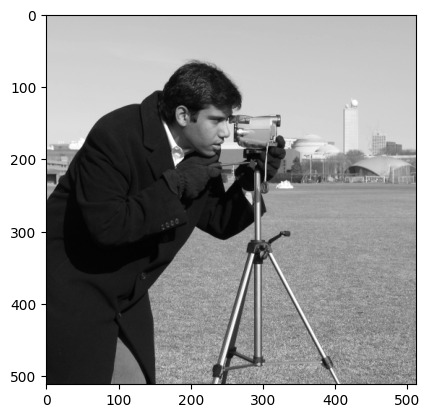
\includegraphics[scale=0.5]{images/7.1.jpg}$$
$$Fig. \; Original \; cameraman \; image $$
$$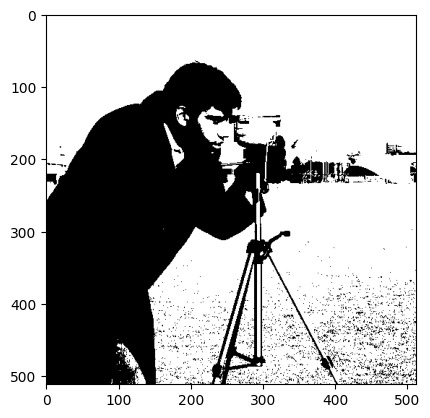
\includegraphics[scale=0.5]{images/7.2.jpg}$$
$$Fig. \; 'Binarized' \; cameraman \; image $$
We, then introduce noise to this ’binarized’ image. In order
to test the capability, we add varying levels of noise, from 5 percent 
to 25 percent of the pixel values.
The varying levels of noises are shown below.
$$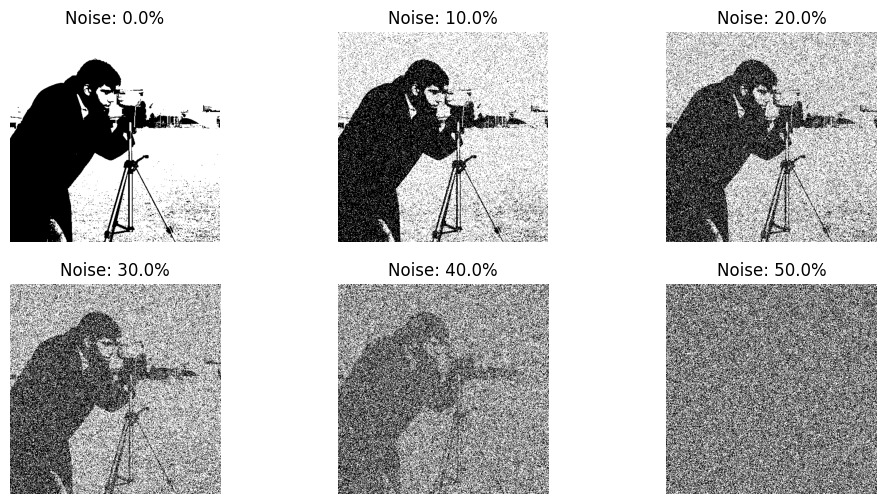
\includegraphics[scale=0.28]{images/7.3.jpg}$$
$Fig. \;  Varying\;  levels \; of\; noise\; added\; in\; the\; cameraman\\image $ \\ \\
Markov random fields sue a quadratic potential function to
measure the energy potential of the image when changing a
particular pixel, with respect to the neighbouring pixels.

This is because for most cases, the values around a pixel
are close to the pixel value. We use the value of
the constant lambdas as -100, while computing the quadratic
potential function.

We ran the algorithm for 5*512*512 = 1310720 iterations.
\section{Part B} 
For the sample code hopfield.m supplied in the lab-work
folder, find out the amount of error (in bits) tolerable for each
of the stored patterns.
$$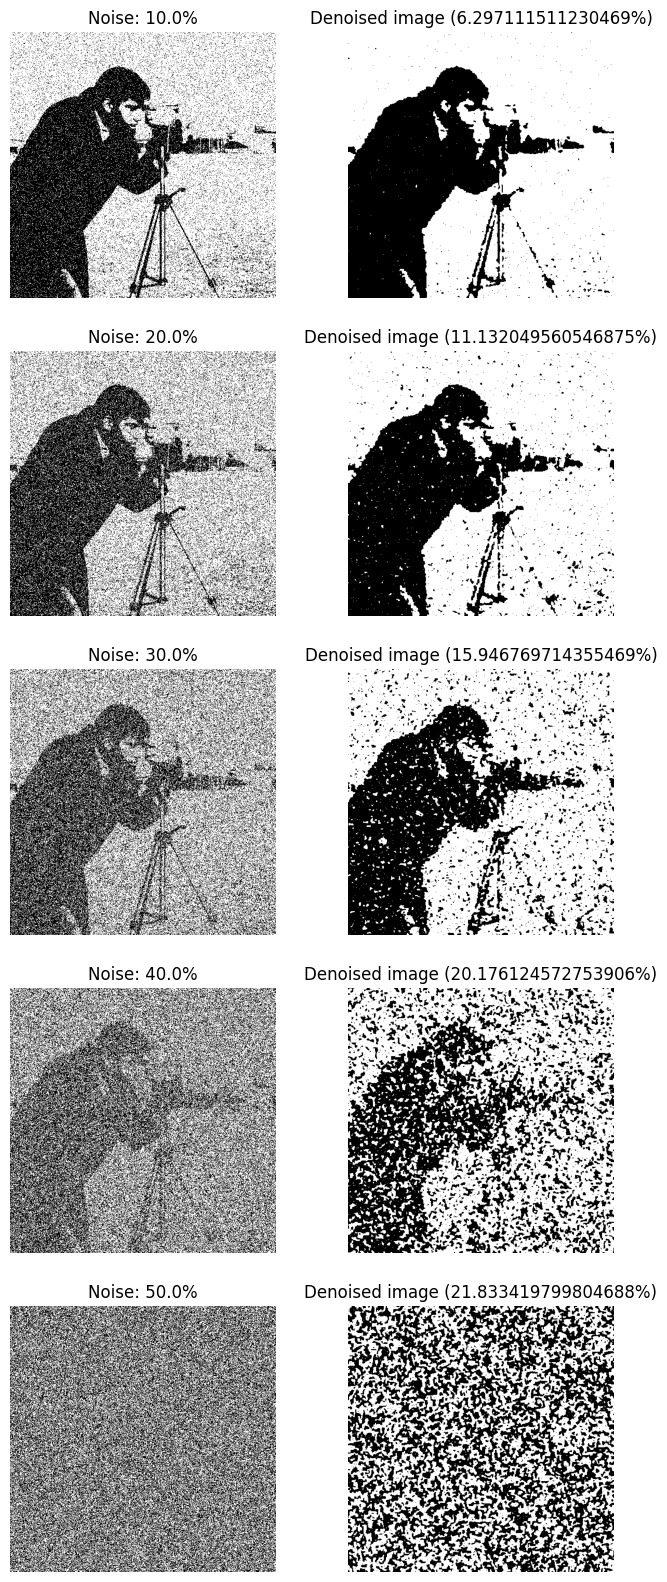
\includegraphics[scale=0.25]{images/7.4.jpg}$$
$$Fig. \; Denoised \; images \; cameraman \; image $$
For this task, we converted the hopfield.m MATLAB codes
to Python so that we could do it in the same Notebook as the
other parts.
The original images looked as shown in fig. below.
$$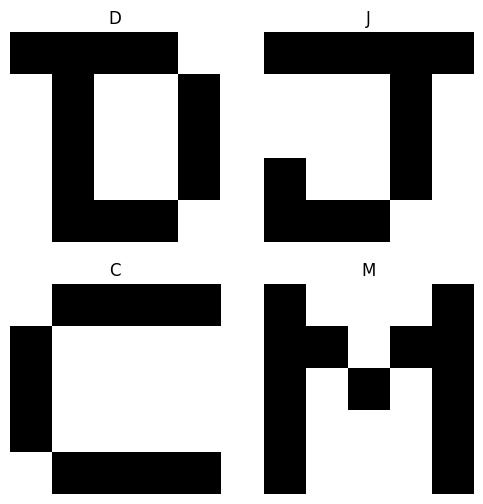
\includegraphics[scale=0.3]{images/7.5.jpg}$$
$$Fig. \; The\; original\; letters\; for\; the\; hopfield\; networks $$
The network was trained using Hebb’s rule, as in the file
and then they were noised by changing some random pixel
values. At max, 15 pixel values were noised.
We can see that suprisingly, the network can correct upto
max 8 errors. The results are show in fig. below.
$$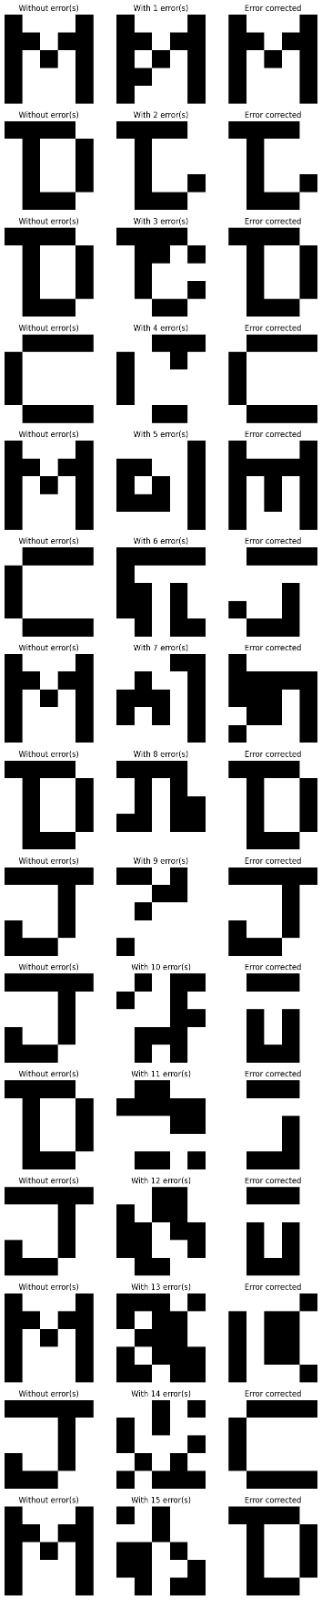
\includegraphics[scale=0.3]{images/7.6.jpg}$$
$$Fig. \;The \; original, \; noised \; and \; conrrected \; letters $$
\section{Part C} 
Solve a TSP (travelling salesman problem) of 10 cities with
a Hopfield network. How many weights do you need for the
network?

This is the usual famous NP-hard problem of Travelling
Salesman, that is done using the a Hopfield Networks.

Since in a Hopfield Netwosk, each node is connected to
each other node, we needed a total of 10x10 = 100 weights.

We first generate 10 cities randomly, as shown in figure below.
$$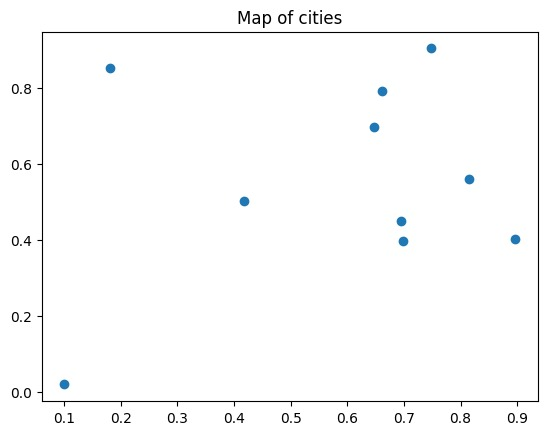
\includegraphics[scale=0.4]{images/7.8.jpg}$$
$$Fig. \; Cities $$

And then let the hopfield network predict an optimal least
path cost.
The path that we got was as shown in figure.
$$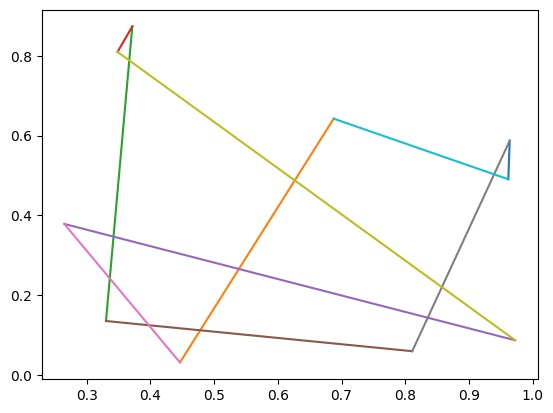
\includegraphics[scale=0.4]{images/7.11.jpg}$$
$$Fig. \; Shortest \; Path $$
\begin{thebibliography}{}
\bibitem{}
CS302-AI Full-House-AI(2023) \href{https://github.com/Full-House-AI/AI-LAB7}{https://github.com/Full-House-AI/AI-LAB7}(2023).
\bibitem{}
What is the reason the test image ”Cameraman” is used widely
to test algorithms in image processing and image encryption?\\
\href{https://www.researchgate.net/post/What_is_the_reason_the_test_image_Cameraman_is_used_widely_to_test_algorithms_in_image_processing_and_image_encryption}{$https://www.researchgate.net/post/What_is_the_reason_the_test_image_Cameraman_is_used_widely_to_test_algorithms_in_image_processing_and_image_encryption$}
\bibitem{}
Image Denoising Benchmark\\
\href{https://www.cs.utoronto.ca/~strider/Denoise/Benchmark/}{https://www.cs.utoronto.ca/~strider/Denoise/Benchmark/}
\bibitem{}
Random Markov Fields\\
\href{https://web.cs.hacettepe.edu.tr/~erkut/bil717.s12/w11a-mrf.pdf}{https://web.cs.hacettepe.edu.tr/~erkut/bil717.s12/w11a-mrf.pdf}
\end{thebibliography}
\end{document}


